% ===================== SymFail (SymTrace) =====================
\subsection{SymFail (SymTrace)}\label{ds:symtrace}
\badgerow{\naturalbadge\ \okbadge\ \lbl{failure node + C1--C4 symptom set}\ \lbl{3 annotators + adjudicator}\ \lbl{MAS, replayable event graphs}\ \lbl{WebArena-Verified Hard / AssistantBench}}

\begin{identity}
Paper & \emph{Repair or Resample? Rethinking Failure Debugging in LLM Multi-Agent Systems} --- Luan, Zhang, Hu, Yang, Yu, Chen (East China Normal Univ., Nanyang Technological Univ., Xi'an Univ.\ of Architecture and Technology), arXiv:2608.25920 (v2, Aug 2026, preprint, no venue) \cite{luan2026symtrace}\\
Links & \href{https://anonymous.4open.science/r/SymTrace-7234}{anonymous review repository \code{SymTrace-7234}} (\code{SymTrace/} replay framework and adapters, \code{SymFail/} data) \textperiodcentered\ no Hugging Face dataset, GitHub repository or project page found (2026-10-26)\\
License & SymFail annotations, trace graphs and metadata CC BY 4.0 (\code{SymFail/DATA\_LICENSE.md}); WebArena / AssistantBench tasks and model outputs keep their own terms; no licence for the code\\
Status & downloaded in full (53 MB zip export, 354 MB extracted): the paper's 536-case package (536 annotations + 536 trace bundles, 2,144 files) and a newer, undocumented 437-case package (3,453 files); \code{data/symtrace/}\\
\end{identity}

\begin{multicols}{2}
\paragraph{Description} SymTrace is an evaluation framework for MAS failure \emph{repair} rather than attribution: it records an execution as an event-dependency graph with boundary logging of every model and tool call, chooses an \emph{intervention anchor} node, rebuilds the prefix from the recorded boundary results under strict matching and lets everything after the anchor run live (``selective replay''). SymFail is the frozen set of source failures the study intervenes on. \textbf{Construction} (natural failures): a deterministic pool of 200 tasks---all 33 eligible AssistantBench dev tasks and the first 167 WebArena-Verified Hard tasks (33 Web-QA, 70 mutation, 25 navigation, 72 retrieval)---each run once with \textbf{AG2}, \textbf{CrewAI} and \textbf{Magentic-One} through SymTrace's instrumented adapters, backbone \code{deepseek-v4-flash} at temperature 0. The native evaluators mark 536 of the 600 runs as failed (462 of 501 WebArena, 74 of 99 AssistantBench): 171 AG2, 184 CrewAI, 181 Magentic-One; the 64 accepted runs are not released. \textbf{Annotation}: four annotators with software-engineering backgrounds; three label independently all applicable categories, one primary category and the \emph{earliest trace-supported actionable node} with evidence and rationale; a fourth reviews everything and fixes the final label with authority to revise (no majority vote). Fleiss' $\kappa$ among the three: 0.62 primary category, 0.57 exact category set, 0.81 node kind (per category C1 0.70, C2 0.37, C3 0.72, C4 0.69); the node is unanimous in 73.9\% of cases and supported by two of three in 95.9\%; the adjudicated label set differs from the union in 21.1\%. \textbf{Taxonomy} (four MAST modes collapsed, explicitly ``intervention signals rather than failure verdicts''): C1 task-constraint violation (FM-1.1), C2 repeated or stalled progress (FM-1.3/1.5), C3 unresolved runtime condition (FM-2.2/2.3 extended to execution and context failures), C4 plan--action--outcome inconsistency (FM-2.6). Labels released: \code{failure\_node\_id}, \code{failure\_node\_kind}, primary label, label set, confidence, the three individual annotations and unanimity flags; rationales and evidence are withheld from the public export, and there is no agent, root-cause or repair label.

\paragraph{Metrics and baselines} No attribution metric: the benchmark measures \emph{reproduction} (rep@$k$, the replayed run fails again) and \emph{repair} (pass@$k$ under the native evaluator). Selective replay reproduces the source failure in 80.8\% of single attempts against 67.97\% for a full rerun (rep@3 52.4 vs 41.4), and 39 of 54 initially successful runs fail at least once in three reruns. Repair pass rate in \% (paper Tables 3--4; task-level methods get three attempts, node-level ones a single selective replay):

\begin{center}\small\setlength{\tabcolsep}{3.5pt}
\begin{tabular}{@{}lccccc@{}}\toprule
Method & att. & AG2 & CrewAI & M-One & Total\\\midrule
Last-Node & 1 & 0.58 & 1.63 & 1.66 & 1.31\\
Random-Node & 1 & 2.34 & 4.89 & 3.87 & 3.73\\
Critic-Agent & 3 & 4.09 & 2.72 & 4.42 & 3.73\\
Self-Reflection & 3 & 4.68 & 2.17 & 6.08 & 4.29\\
Unguided Full Rerun & 3 & 8.19 & 3.80 & 8.84 & 6.90\\
Suspicious-Node (theirs) & 1 & \textbf{16.37} & \textbf{25.00} & \textbf{18.78} & \textbf{20.15}\\\bottomrule
\end{tabular}
\end{center}
The anchor comes from a rule + LLM \emph{suspicious-node} score (fused 0.55/0.45, gate 0.5, hand-set) and the repair prompt is conditioned on the C1--C4 label. One intervention costs 10--15 API calls per repair.

\paragraph{Schema} \code{human\_annotations\_536.jsonl}: one object per case with \code{task\_id} (\code{webarena\_verified\_hard\_<n>} / \code{assistantbench\_dev\_<hash>}), \code{mas}, \code{failure\_node\_id} (\code{<task>:attempt\_000:snapshot:<hash>:<node>}), \code{failure\_node\_kind}, \code{primary\_failure\_label}, \code{failure\_labels}, \code{confidence}, \code{inter\_annotator\_agreement} and \code{individual\_annotations}. One bundle per case in \code{initial\_failure\_logs\_536/<mas>/<task\_id>/attempt\_000/}: \code{graph.json} (\code{masd.graph.v1}: \code{nodes} with \code{kind} $\in$ \{\code{sys\_prompt}, \code{user\_input}, \code{agent\_action}, \code{tool\_call}, \code{tool\_result}, \code{final\_result}, \code{error}\}, \code{agent\_id}, \code{action}, \code{observation}, \code{tool\_call}, \code{tool\_result}, \code{final\_answer} and the full \code{api\_messages} / \code{api\_response} of LLM-backed actions; \code{edges} with a dependency \code{reason}; \code{topological\_order}; \code{capture\_summary}), \code{trajectory.json} (nodes + run result + task with reference answer or WebArena evaluator spec), \code{result\_record.json} (\code{final\_answer}, \code{evaluator\_evidence}, latency, model) and \code{api\_records.jsonl} (request, response, usage per LLM call). We take one node in \code{topological\_order} as one step (node 0 is the system prompt, node 1 the task).
\end{multicols}

\paragraph{Statistics} computed from the downloaded 536-case package.\par\nobreak\vspace{1pt}
\noindent\begin{minipage}[t]{0.58\linewidth}\vspace{0pt}\small
{\footnotesize\setlength{\tabcolsep}{3.5pt}\fitbox{\begin{tabular}{@{}lrrrr@{}}\toprule
 & All & AG2 & CrewAI & Magentic-One\\\midrule
trajectories (all failed) & 536 & 171 & 184 & 181\\
WebArena-V.\ Hard / AssistantBench & 462 / 74 & 146 / 25 & 161 / 23 & 155 / 26\\
graph nodes: mean / median & 10.4 / 7 & 10.4 / 13 & 7.7 / 5 & 13.0 / 7\\
graph nodes: min -- max & 5 -- 21 & 5 -- 15 & 5 -- 15 & 7 -- 21\\
LLM calls: mean (max 3) & 1.9 & 2.2 & 1.6 & 1.9\\
failure node index: mean / median & 3.8 / 3 & 5.8 / 4 & 3.1 / 2 & 2.7 / 2\\
relative position: mean / median & 0.49 / 0.50 & 0.71 / 0.79 & 0.49 / 0.50 & 0.28 / 0.33\\
failure node = \code{final\_result} & 98 & 82 & 15 & 1\\
primary C1 / C2 / C3 / C4 & 125 / 69 / 203 / 139 & 37 / 2 / 72 / 60 & 49 / 21 / 36 / 78 & 39 / 46 / 95 / 1\\
characters / traj.: mean / median & 5.5\,k / 3.6\,k & 3.3\,k / 2.8\,k & 2.7\,k / 1.9\,k & 10.5\,k / 9.1\,k\\
failed tool results (total) & 377 & 168 & 77 & 132\\\bottomrule
\end{tabular}}}

\smallskip 194 distinct tasks, 155 of which fail under all three MAS. Label sets are large: mean 2.77 labels per case, C4 present in 87\% and C1 in 82\%, all four in 91 cases. Node kinds over the corpus: 2,726 \code{agent\_action}, 607 \code{tool\_call} + 607 \code{tool\_result}, 536 final results. 276 trajectories make a single LLM call and no tool call; 173 WebArena runs fail on the literal site placeholder (\code{\_\_SHOPPING\_\_}: \code{MissingSchema} / \code{NameResolutionError}), only 23 of 462 WebArena runs contain one successful fetch, and the evaluator records \code{has\_real\_tool\_event: false} for 447 of them; all 74 AssistantBench runs did reach the live web. 148 final answers declare that the task could not be completed. Agent id of the failure node: \code{crewai} 184, \code{ag2} 166, \code{user} 102 (Magentic-One's echo of the task), \code{masd\_magnetic\_one\_assistant} 77. Mean wall-clock 17\,s per run; \code{token\_usage} is empty in every record.
\end{minipage}\hfill
\begin{minipage}[t]{0.40\linewidth}\vspace{0pt}
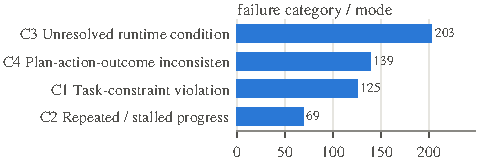
\includegraphics[width=\linewidth]{3_core/symtrace/figures/cat.pdf}
\end{minipage}

\paragraph{Example trajectory} AG2 run \code{webarena\_verified\_hard\_96} (13 graph nodes, 3 LLM calls, 2.6\,k characters): the shortest trajectory with a tool call whose unanimous failure node is an action before the final answer. The agent browses the literal placeholder \code{\_\_SHOPPING\_\_}, receives \code{MissingSchema}, retries with \code{https://\_\_SHOPPING\_\_} (node 7, primary C3, all four labels), receives a DNS failure and answers ``status unknown''; the evaluator expected ``canceled''. The record illustrates both the failure-node convention (the retry that continues from an unresolved condition, not the final answer) and the environment problem discussed below.
% auto-generated by scripts/render_traj.py -- do not edit
\trajtask{initial\_failure\_logs\_536/\allowbreak{}ag2/\allowbreak{}webarena\_verified\_hard\_96}{Get the status of my latest order and when will it arrive. Return a list of objects with keys "status" and "arrival\_date" (YYYY-MM-DD format or null if not available),\allowbreak{} without any additional details.}
\begin{trajstep}{0}{ag2 [sys\_prompt]}{agA}
MASD controlled experiment prompt and adapter constraints.
\end{trajstep}
\begin{trajstep}{1}{user [user\_input]}{agB}
Mode:\allowbreak{} snapshot\newline Task id:\allowbreak{} webarena\_verified\_hard\_96\newline Benchmark:\allowbreak{} webarena\_verified /\allowbreak{} hard\newline Task:\allowbreak{} Get the status of my latest order and when will it arrive. Return a list of objects with keys "status" and "arrival\_date" (YYYY-MM-DD format or null if not available),\allowbreak{} without any additional details.\newline Start URLs or tools:\allowbreak{} ['\_\_SHOPPING\_\_']\newline Return only the final answer and a short note about what evidence would be needed.
\end{trajstep}
\begin{trajstep}{2}{masd\_ag2\_multistep\_assistant [agent\_action]}{agC}
[ag2\_process\_message\_before\_send] \{"action":\allowbreak{}"browse",\allowbreak{}"url":\allowbreak{}"\_\_SHOPPING\_\_",\allowbreak{}"reason":\allowbreak{}"Start at the shopping site to access account and view latest order status."\}
\end{trajstep}
\begin{trajstep}{3}{ag2 [agent\_action]}{agD}
[ag2\_agent\_step] \{"action":\allowbreak{}"browse",\allowbreak{}"url":\allowbreak{}"\_\_SHOPPING\_\_",\allowbreak{}"reason":\allowbreak{}"Start at the shopping site to access account and view latest order status."\}
\end{trajstep}
\begin{trajstep}{4}{ag2 [tool\_call]}{agE}
\{"reason":\allowbreak{} "Start at the shopping site to access account and view latest order status.",\allowbreak{} "type":\allowbreak{} "browser\_http\_get",\allowbreak{} "url":\allowbreak{} "\_\_SHOPPING\_\_"\}
\end{trajstep}
\begin{trajstep}{5}{browser\_tool [tool\_result]}{agF}
\{'type':\allowbreak{} 'browser\_http\_get',\allowbreak{} 'status':\allowbreak{} 'failed',\allowbreak{} 'url':\allowbreak{} '\_\_SHOPPING\_\_',\allowbreak{} 'latency':\allowbreak{} 0.0015594959259033203,\allowbreak{} 'error':\allowbreak{} \{'type':\allowbreak{} 'MissingSchema',\allowbreak{} 'message':\allowbreak{} "Invalid URL '\_\_SHOPPING\_\_':\allowbreak{} No scheme supplied. Perhaps you meant https:\allowbreak{}/\allowbreak{}/\allowbreak{}\_\_SHOPPING\_\_"\}\}
\end{trajstep}
\begin{trajstep}{6}{masd\_ag2\_multistep\_assistant [agent\_action]}{agC}
[ag2\_process\_message\_before\_send] \{"action":\allowbreak{}"browse",\allowbreak{}"url":\allowbreak{}"https:\allowbreak{}/\allowbreak{}/\allowbreak{}\_\_SHOPPING\_\_",\allowbreak{}"reason":\allowbreak{}"Need to access the shopping site. The placeholder needs a scheme."\}
\end{trajstep}
\begin{faultystep}{7}{ag2 [agent\_action]}{agD}
[ag2\_agent\_step] \{"action":\allowbreak{}"browse",\allowbreak{}"url":\allowbreak{}"https:\allowbreak{}/\allowbreak{}/\allowbreak{}\_\_SHOPPING\_\_",\allowbreak{}"reason":\allowbreak{}"Need to access the shopping site. The placeholder needs a scheme."\}
\end{faultystep}
\begin{trajstep}{8}{ag2 [tool\_call]}{agE}
\{"reason":\allowbreak{} "Need to access the shopping site. The placeholder needs a scheme.",\allowbreak{} "type":\allowbreak{} "browser\_http\_get",\allowbreak{} "url":\allowbreak{} "https:\allowbreak{}/\allowbreak{}/\allowbreak{}\_\_SHOPPING\_\_"\}
\end{trajstep}
\begin{trajstep}{9}{browser\_tool [tool\_result]}{agF}
\{'type':\allowbreak{} 'browser\_http\_get',\allowbreak{} 'status':\allowbreak{} 'failed',\allowbreak{} 'url':\allowbreak{} 'https:\allowbreak{}/\allowbreak{}/\allowbreak{}\_\_SHOPPING\_\_',\allowbreak{} 'latency':\allowbreak{} 7.287393808364868,\allowbreak{} 'error':\allowbreak{} \{'type':\allowbreak{} 'ConnectionError',\allowbreak{} 'message':\allowbreak{} 'HTTPSConnectionPool(host=\allowbreak{}\textbackslash{}'\_\_shopping\_\_\textbackslash{}',\allowbreak{} port=\allowbreak{}443):\allowbreak{} Max retries exceeded with url:\allowbreak{} /\allowbreak{} (Caused by NameResolutionError("HTTPSConnection(host=\allowbreak{}\textbackslash{}'\_\_shopping\_\_\textbackslash{}',\allowbreak{} port=\allowbreak{}443):\allowbreak{} Failed to resolve \textbackslash{}'\_\_shopping\_\_\textbackslash{}' ([Errno 11001] getaddrinfo failed)"))'\}\}
\end{trajstep}
\begin{trajstep}{10}{masd\_ag2\_multistep\_assistant [agent\_action]}{agC}
[ag2\_process\_message\_before\_send] \{"final":\allowbreak{}"[\textbackslash{}n \{\textbackslash{}"status\textbackslash{}":\allowbreak{} \textbackslash{}"unknown\textbackslash{}",\allowbreak{} \textbackslash{}"arrival\_date\textbackslash{}":\allowbreak{} null\}\textbackslash{}n]\textbackslash{}n\textbackslash{}nNote:\allowbreak{} Evidence needed would be the user's order history page on the shopping site after authentication."\}
\end{trajstep}
\begin{trajstep}{11}{ag2 [agent\_action]}{agD}
[ag2\_agent\_step] \{"final":\allowbreak{}"[\textbackslash{}n \{\textbackslash{}"status\textbackslash{}":\allowbreak{} \textbackslash{}"unknown\textbackslash{}",\allowbreak{} \textbackslash{}"arrival\_date\textbackslash{}":\allowbreak{} null\}\textbackslash{}n]\textbackslash{}n\textbackslash{}nNote:\allowbreak{} Evidence needed would be the user's order history page on the shopping site after authentication."\}
\end{trajstep}
\begin{trajstep}{12}{ag2 [final\_result]}{agG}
[\newline \{"status":\allowbreak{} "unknown",\allowbreak{} "arrival\_date":\allowbreak{} null\}\newline ]\par Note:\allowbreak{} Evidence needed would be the user's order history page on the shopping site after authentication.
\end{trajstep}
\trajannotation{ag2}{7}{C3 Unresolved runtime condition (primary);\allowbreak{} label set \{C1,\allowbreak{} C2,\allowbreak{} C3,\allowbreak{} C4\}}{(annotation rationales and evidence excerpts are withheld from the public export:\allowbreak{} annotation\_prose\_in\_public\_export =\allowbreak{} false;\allowbreak{} the label is the earliest trace-supported actionable node carrying the symptom)}{[\{'evaluator':\allowbreak{} 'AgentResponseEvaluator',\allowbreak{} 'expected':\allowbreak{} \{'error\_details':\allowbreak{} None,\allowbreak{} 'retrieved\_data':\allowbreak{} [\{'arrival\_date':\allowbreak{} None,\allowbreak{} 'status':\allowbreak{} 'canceled'\}],\allowbreak{} 'status':\allowbreak{} 'SUCCESS',\allowbreak{} 'task\_type':\allowbreak{} 'RETRIEVE'\},\allowbreak{} 'ordered':\allowbreak{} False,\allowbreak{} 'results\newline [...] (74 chars omitted) [...]\newline pe':\allowbreak{} 'string'\},\allowbreak{} 'status':\allowbreak{} \{'type':\allowbreak{} 'string'\}\},\allowbreak{} 'type':\allowbreak{} 'object'\},\allowbreak{} 'type':\allowbreak{} 'array'\}\}]}{[\newline \{"status":\allowbreak{} "unknown",\allowbreak{} "arrival\_date":\allowbreak{} null\}\newline ]\par Note:\allowbreak{} Evidence needed would be the user's order history page on the shopping site after authentication.}{\textbf{mas}: AG2; \textbf{source\_benchmark}: WebArena-Verified Hard; \textbf{task\_type}: retrieve; \textbf{difficulty}: hard; \textbf{failure\_node\_id}: agent\_action\_0001; \textbf{failure\_node\_kind}: agent\_action; \textbf{confidence}: high; \textbf{inter\_annotator\_agreement}: \{"annotation\_count":\allowbreak{} 3,\allowbreak{} "primary\_failure\_label\_unanimous":\allowbreak{} true,\allowbreak{} "failure\_label\_set\_unanimous":\allowbreak{} false,\allowbreak{} "failure\_node\_unanimous":\allowbreak{} true,\allowbreak{} "failure\_node\_kind\_unanimous":\allowbreak{} true,\allowbreak{} "strict\_annotation\_unanimous":\allowbreak{} false,\allowbreak{} "final\_primary\_failure\_label\_support\_count":\allowbreak{} 0,\allowbreak{} "final\_failure\_label\_set\_support\_count":\allowbreak{} 1,\allowbreak{} "final\_failure\_node\_support\_count":\allowbreak{} 3,\allowbreak{} "final\_strict\_annotation\_support\_count":\allowbreak{} 0\}; \textbf{evaluator\_evidence}: \{"evaluator\_names":\allowbreak{} ["AgentResponseEvaluator"],\allowbreak{} "expected\_retrieved\_data":\allowbreak{} [\{"arrival\_date":\allowbreak{} null,\allowbreak{} "status":\allowbreak{} "canceled"\}],\allowbreak{} "has\_real\_tool\_event":\allowbreak{} false,\allowbreak{} "method":\allowbreak{} "webarena\_verified\_evaluator",\allowbreak{} "missing\_retrieved\_data":\allowbreak{} [\{"expected":\allowbreak{} \{"arrival\_date":\allowbreak{} null,\allowbreak{} "status":\allowbreak{} "canceled"\},\allowbreak{} "missing\_values":\allowbreak{} ["None",\allowbreak{} "canceled"]\}],\allowbreak{} "observed\_answer\_excerpt":\allowbreak{} "[\textbackslash{}n \{\textbackslash{}"st\newline [...] (506 chars omitted) [...]\newline tus":\allowbreak{} "failed",\allowbreak{} "type":\allowbreak{} "browser\_http\_get",\allowbreak{} "url":\allowbreak{} "https:\allowbreak{}/\allowbreak{}/\allowbreak{}\_\_SHOPPING\_\_"\},\allowbreak{} "requires\_environment\_event":\allowbreak{} false,\allowbreak{} "task\_types":\allowbreak{} ["RETRIEVE"]\}; \textbf{llm\_call\_count}: 3; \textbf{tool\_failure\_count}: 2; \textbf{step\_indexing}: 0-based position of the node in graph.json topological\_order (sys\_prompt =\allowbreak{} 0,\allowbreak{} user\_input =\allowbreak{} 1)}


\paragraph{Notes} (i) \emph{Replayable by construction}: every bundle holds the full event graph with per-call LLM requests and responses and tool boundary results, and the repository ships the code that replays a prefix from them---the closest released analogue to TraceElephant's dynamic setting (\S\ref{ds:traceelephant}) and the operational form of the rollouts in Section~\ref{sec:future:perturb}; CrewAI appears in no other dataset here. (ii) \emph{Thin adapters, tiny budget}: the ``MAS'' are SymTrace's \code{masd\_*} adapters (one assistant plus a \code{browser\_http\_get} tool) capped at three LLM calls; graph sizes are nearly constant per framework and the median run has one LLM call. Agent-level attribution is meaningless---the failure node's agent is the framework name, the assistant or \code{user}. (iii) \emph{Most WebArena runs never reached the environment}: the site placeholders were not substituted in the released runs, so the bulk of the 462 WebArena failures are the agent answering, or declaring inability, without page content; this is what C3 (38\%) and C4 record, and it should be kept in mind when reading the 20\% repair rate. (iv) \emph{Symptoms, not root causes}: C1--C4 are intervention signals by the authors' own description; the informative targets are the primary label ($\kappa$ 0.62) and the node (73.9\% unanimous), which is the first agent action in 246 cases and the final node in 98. (v) \emph{Incomplete public export}: rationales and evidence withheld, token usage empty, successful runs absent, anonymous hosting. The 437-case package (six frameworks including ChatDev, MetaGPT and OpenManus on ProgramDev; GPT, Claude and Gemini backbones) is a different, single-reviewer study whose failure node is \code{node\_final} in every case and whose reasons are five template strings---not a step-labelled resource. (vi) \emph{Overlaps}: Magentic-One and AssistantBench with Who\&When, TraceElephant and AgentRx (new runs, different backbone); WebArena with LongRCA and HORIZON; the taxonomy maps onto MAST (\S\ref{ds:mast_data}).
